\documentclass[english]{SPFShortReport}
\usepackage{subfigure}
\usepackage{spfFigures}
\usepackage{longtable}
\usepackage{url}
\usepackage{gensymb}
\usepackage[yyyymmdd,hhmmss]{datetime}
\reportName{Python calculation for heat pump SIN-50TU}
\reportSubName{Parametric Heat Pump calculation} 
\reportDate{\today \hspace{0.1cm} at: \currenttime \hspace{0.1cm} h} 
\author{Dani Carbonell}
\address{dani.carbonell@solarenergy.ch}
\begin{document}
\begin{table}[!ht]
\begin{small}
\caption{Fitted coefficients for the heat pump.}
\begin{center}
\resizebox{12cm}{!} 
{
\begin{tabular}{l | c c } 
\hline
\hline
Coefficient &Description & \\ 
 & &$[kW]$\\ 
\hline
$PQ_{1}$ & \emph{$1^{st}$ condenser polynomial coefficient}  & 4.5713e+01    \\ 
$PQ_{2}$ & \emph{$2^{st}$ condenser polynomial coefficient}  & 5.3253e+02    \\ 
$PQ_{3}$ & \emph{$3^{st}$ condenser polynomial coefficient}  & 2.1462e+02    \\ 
$PQ_{4}$ & \emph{$4^{st}$ condenser polynomial coefficient}  & -6.8035e+02    \\ 
$PQ_{5}$ & \emph{$5^{st}$ condenser polynomial coefficient}  & 7.1420e+02    \\ 
$PQ_{6}$ & \emph{$6^{st}$ condenser polynomial coefficient}  & -1.0875e+03    \\ 
\hline
$PCOP_{1}$ & \emph{$1^{st}$ COP polynomial coefficient}  & 6.5443e+00    \\ 
$PCOP_{2}$ & \emph{$2^{st}$ COP polynomial coefficient}  & 6.2672e+01    \\ 
$PCOP_{3}$ & \emph{$3^{st}$ COP polynomial coefficient}  & 3.1491e+00    \\ 
$PCOP_{4}$ & \emph{$4^{st}$ COP polynomial coefficient}  & -1.6528e+02    \\ 
$PCOP_{5}$ & \emph{$5^{st}$ COP polynomial coefficient}  & 1.7388e+02    \\ 
$PCOP_{6}$ & \emph{$6^{st}$ COP polynomial coefficient}  & -1.1522e+02    \\ 
\hline
$\dot m_{cond}$ & 8800.00 $[kg/h]$\\ 
$\dot m_{evap}$ & 8800.00 $[kg/h]$\\ 
\hline
$COP_{nom}$ (B0W35)& 4.95 \\ 
$Q_{c,nom}$ (B0W35)& 52.22 kW\\ 
$COP_{nom}$ (B2W35)& 5.24 \\ 
$Q_{c,nom}$ (B2W35)& 55.23 kW\\ 
$COP_{nom}$ (B10W35)& 6.57 \\ 
$Q_{c,nom}$ (B10W35)& 67.91 kW\\ 
\hline
\hline
\end{tabular}
}
\label{CoefTable}
\end{center}
\end{small}
\end{table}
\begin{table}[!ht]
\begin{small}
\caption{Predicting results of the heat pump.}
\begin{center}
\resizebox{12cm}{!} 
{
\begin{tabular}{l | c c c c c c c c c c c } 
\hline
\hline
$T_{evap,in}$ &$T_{evap,out}$ &$T_{cond,in}$ &$T_{cond,out}$ &$COP$ &$Q_{cond}$ &$Q_{evap}$ &$W_{comp}$ &$\dot m_{cond}$ &$\dot m_{evap}$ &$\Delta T_{evap}$ &$\Delta T_{cond}$ \\ 
$^oC$ &$^oC$ &$^oC$ &$^oC$ &$[-]$ &$[kW]$ &$[kW]$ &$[kW]$ &kg/h &kg/h &K &K\\ 
\hline
-7.00 & -10.49 & 25.88 & 30.00 & 4.37 & 42.20 & 32.55 & 9.65 & 8800 & 8800 & 3.5 & 4.1\\ 
-7.00 & -10.29 & 34.68 & 38.75 & 3.78 & 41.67 & 30.65 & 11.02 & 8800 & 8800 & 3.3 & 4.1\\ 
-7.00 & -9.77 & 43.69 & 47.50 & 2.95 & 39.05 & 25.80 & 13.25 & 8800 & 8800 & 2.8 & 3.8\\ 
-7.00 & -8.71 & 52.89 & 56.25 & 1.87 & 34.37 & 15.95 & 18.42 & 8800 & 8800 & 1.7 & 3.4\\ 
-7.00 & -4.85 & 62.17 & 65.00 & 0.59 & 28.96 & -20.06 & 49.03 & 8800 & 8800 & -2.2 & 2.8\\ 
-4.00 & -7.94 & 25.46 & 30.00 & 4.76 & 46.51 & 36.73 & 9.78 & 8800 & 8800 & 3.9 & 4.5\\ 
-4.00 & -7.72 & 34.28 & 38.75 & 4.12 & 45.83 & 34.69 & 11.13 & 8800 & 8800 & 3.7 & 4.5\\ 
-4.00 & -7.19 & 43.30 & 47.50 & 3.24 & 43.05 & 29.75 & 13.30 & 8800 & 8800 & 3.2 & 4.2\\ 
-4.00 & -6.15 & 52.52 & 56.25 & 2.11 & 38.20 & 20.10 & 18.10 & 8800 & 8800 & 2.2 & 3.7\\ 
-4.00 & -3.02 & 61.85 & 65.00 & 0.78 & 32.21 & -9.11 & 41.33 & 8800 & 8800 & -1.0 & 3.1\\ 
-1.00 & -5.41 & 25.03 & 30.00 & 5.18 & 50.95 & 41.11 & 9.84 & 8800 & 8800 & 4.4 & 5.0\\ 
-1.00 & -5.18 & 33.86 & 38.75 & 4.49 & 50.12 & 38.96 & 11.16 & 8800 & 8800 & 4.2 & 4.9\\ 
-1.00 & -4.64 & 42.89 & 47.50 & 3.56 & 47.19 & 33.95 & 13.24 & 8800 & 8800 & 3.6 & 4.6\\ 
-1.00 & -3.63 & 52.13 & 56.25 & 2.39 & 42.17 & 24.55 & 17.62 & 8800 & 8800 & 2.6 & 4.1\\ 
-1.00 & -1.02 & 61.51 & 65.00 & 1.01 & 35.71 & 0.23 & 35.48 & 8800 & 8800 & 0.0 & 3.5\\ 
2.00 & -2.90 & 24.58 & 30.00 & 5.63 & 55.54 & 45.68 & 9.86 & 8800 & 8800 & 4.9 & 5.4\\ 
2.00 & -2.66 & 33.42 & 38.75 & 4.90 & 54.56 & 43.42 & 11.13 & 8800 & 8800 & 4.7 & 5.3\\ 
2.00 & -2.11 & 42.47 & 47.50 & 3.93 & 51.47 & 38.38 & 13.10 & 8800 & 8800 & 4.1 & 5.0\\ 
2.00 & -1.13 & 51.73 & 56.25 & 2.71 & 46.28 & 29.22 & 17.06 & 8800 & 8800 & 3.1 & 4.5\\ 
2.00 & 1.10 & 61.15 & 65.00 & 1.27 & 39.43 & 8.44 & 30.99 & 8800 & 8800 & 0.9 & 3.9\\ 
5.00 & -0.41 & 24.12 & 30.00 & 6.13 & 60.26 & 50.43 & 9.84 & 8800 & 8800 & 5.4 & 5.9\\ 
5.00 & -0.15 & 32.98 & 38.75 & 5.35 & 59.13 & 48.08 & 11.06 & 8800 & 8800 & 5.2 & 5.8\\ 
5.00 & 0.39 & 42.04 & 47.50 & 4.33 & 55.90 & 43.00 & 12.90 & 8800 & 8800 & 4.6 & 5.5\\ 
5.00 & 1.35 & 51.32 & 56.25 & 3.07 & 50.54 & 34.08 & 16.46 & 8800 & 8800 & 3.7 & 4.9\\ 
5.00 & 3.30 & 60.77 & 65.00 & 1.58 & 43.36 & 15.87 & 27.49 & 8800 & 8800 & 1.7 & 4.2\\ 
8.00 & 2.07 & 23.64 & 30.00 & 6.66 & 65.13 & 55.34 & 9.78 & 8800 & 8800 & 5.9 & 6.4\\ 
8.00 & 2.33 & 32.52 & 38.75 & 5.83 & 63.85 & 52.90 & 10.94 & 8800 & 8800 & 5.7 & 6.2\\ 
8.00 & 2.88 & 41.60 & 47.50 & 4.77 & 60.46 & 47.80 & 12.67 & 8800 & 8800 & 5.1 & 5.9\\ 
8.00 & 3.81 & 50.89 & 56.25 & 3.47 & 54.94 & 39.09 & 15.85 & 8800 & 8800 & 4.2 & 5.4\\ 
8.00 & 5.56 & 60.36 & 65.00 & 1.92 & 47.48 & 22.76 & 24.72 & 8800 & 8800 & 2.4 & 4.6\\ 
11.00 & 4.52 & 23.15 & 30.00 & 7.22 & 70.13 & 60.42 & 9.71 & 8800 & 8800 & 6.5 & 6.8\\ 
11.00 & 4.79 & 32.04 & 38.75 & 6.36 & 68.71 & 57.90 & 10.81 & 8800 & 8800 & 6.2 & 6.7\\ 
11.00 & 5.34 & 41.14 & 47.50 & 5.25 & 65.17 & 52.76 & 12.41 & 8800 & 8800 & 5.7 & 6.4\\ 
11.00 & 6.26 & 50.44 & 56.25 & 3.90 & 59.49 & 44.23 & 15.26 & 8800 & 8800 & 4.7 & 5.8\\ 
11.00 & 7.86 & 59.94 & 65.00 & 2.30 & 51.77 & 29.30 & 22.48 & 8800 & 8800 & 3.1 & 5.1\\ 
14.00 & 6.96 & 22.65 & 30.00 & 7.83 & 75.27 & 65.65 & 9.62 & 8800 & 8800 & 7.0 & 7.3\\ 
14.00 & 7.24 & 31.55 & 38.75 & 6.91 & 73.70 & 63.04 & 10.66 & 8800 & 8800 & 6.8 & 7.2\\ 
14.00 & 7.80 & 40.66 & 47.50 & 5.76 & 70.03 & 57.88 & 12.15 & 8800 & 8800 & 6.2 & 6.8\\ 
14.00 & 8.69 & 49.98 & 56.25 & 4.37 & 64.18 & 49.49 & 14.69 & 8800 & 8800 & 5.3 & 6.3\\ 
14.00 & 10.18 & 59.51 & 65.00 & 2.72 & 56.25 & 35.60 & 20.64 & 8800 & 8800 & 3.8 & 5.5\\ 
17.00 & 9.39 & 22.14 & 30.00 & 8.47 & 80.54 & 71.03 & 9.51 & 8800 & 8800 & 7.6 & 7.9\\ 
17.00 & 9.67 & 31.05 & 38.75 & 7.51 & 78.84 & 68.34 & 10.50 & 8800 & 8800 & 7.3 & 7.7\\ 
17.00 & 10.23 & 40.18 & 47.50 & 6.32 & 75.02 & 63.14 & 11.88 & 8800 & 8800 & 6.8 & 7.3\\ 
17.00 & 11.12 & 49.51 & 56.25 & 4.88 & 69.03 & 54.87 & 14.16 & 8800 & 8800 & 5.9 & 6.7\\ 
17.00 & 12.52 & 59.06 & 65.00 & 3.18 & 60.88 & 41.77 & 19.12 & 8800 & 8800 & 4.5 & 5.9\\ 
20.00 & 11.79 & 21.61 & 30.00 & 9.14 & 85.95 & 76.55 & 9.40 & 8800 & 8800 & 8.2 & 8.4\\ 
20.00 & 12.09 & 30.54 & 38.75 & 8.14 & 84.12 & 73.78 & 10.33 & 8800 & 8800 & 7.9 & 8.2\\ 
20.00 & 12.65 & 39.67 & 47.50 & 6.90 & 80.16 & 68.55 & 11.61 & 8800 & 8800 & 7.3 & 7.8\\ 
20.00 & 13.53 & 49.02 & 56.25 & 5.42 & 74.01 & 60.36 & 13.66 & 8800 & 8800 & 6.5 & 7.2\\ 
20.00 & 14.87 & 58.59 & 65.00 & 3.68 & 65.69 & 47.85 & 17.84 & 8800 & 8800 & 5.1 & 6.4\\ 
\hline
\hline
\end{tabular}
}
\label{ResultsTable}
\end{center}
\end{small}
\end{table}
\begin{figure}[!ht]
\begin{center}
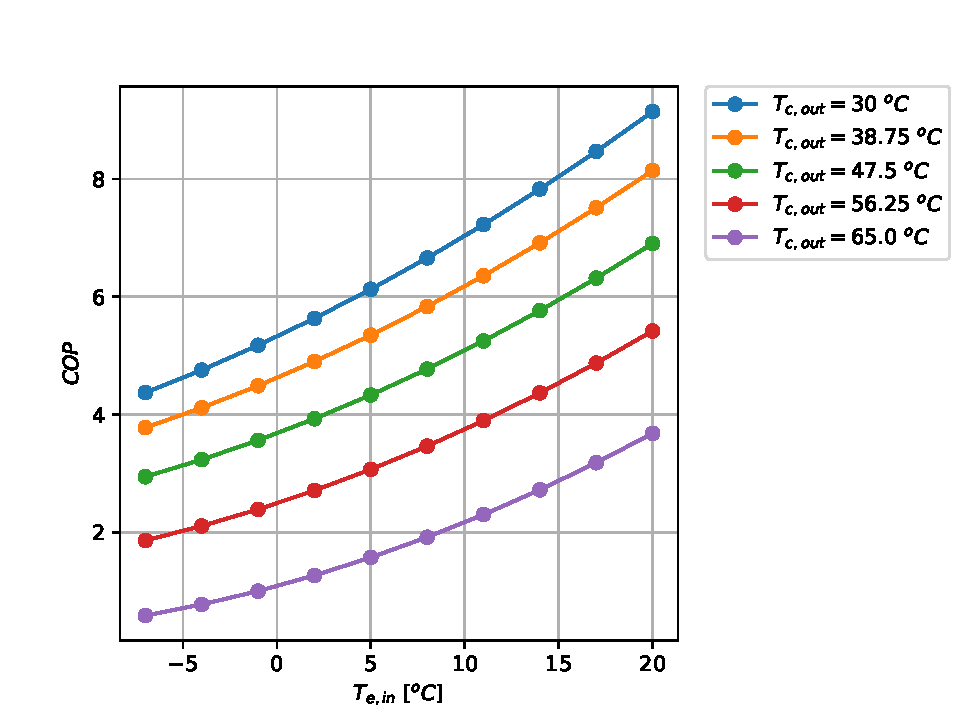
\includegraphics[width=1\textwidth]{C:/Daten/spfPackages/GIT/spfTrnsysFiles/HeatPump/BrineToWater/Walter Meier/SIN-50TU/SIN-50TU-Cop.pdf}
\caption{COP Results for the heat pump at the selected points}
\label{COPFig}
\end{center}
\end{figure}
\begin{figure}[!ht]
\begin{center}
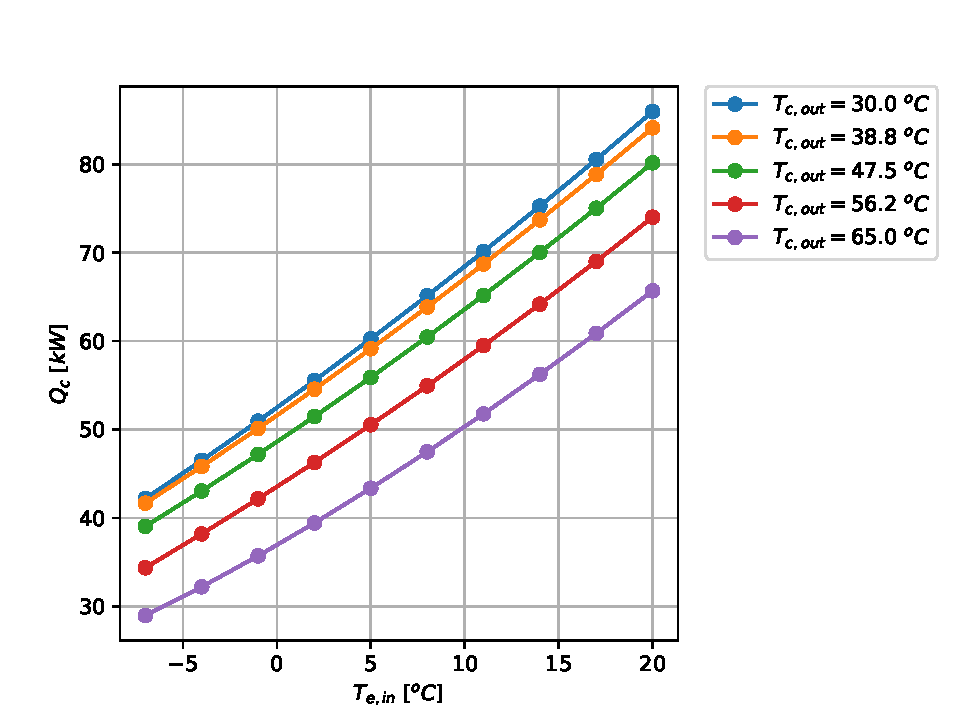
\includegraphics[width=1\textwidth]{C:/Daten/spfPackages/GIT/spfTrnsysFiles/HeatPump/BrineToWater/Walter Meier/SIN-50TU/SIN-50TU-Qc.pdf}
\caption{$Q_c$ Results for the heat pump at the selected points}
\label{QcFig}
\end{center}
\end{figure}
\end{document}
